\part{Análisis de requisitos}

\section{Introducción}

En todos los modelos de ciclos de vida existe la fase de \textbf{análisis de requisitos}, en la cual se estudian las características y funciones del sistema, la definición de los requisitos del software y del sistema del que forma parte, la planificación inicial del proyecto, y tareas de análisis de riesgos. Este análisis se centra en la \uline{información, funcional y de comportamiento del problema}, el cual se divide en partes que se modelan para comprenderlo mejor, con el objetivo de desarrollar una \textbf{especificación de requisitos}, en donde se describe el problema analizado y la solución propuesta.\\

Como se puede prever, esta especificación se convierte en base de todas las actividades que siguen y, por ende, tiene una gran influencia en la calidad de la solución implementada finalmente. El principal problema es que, \uline{al inicio de un proyecto, es difícil tener una idea clara y segura de los requisitos del sistema y del software}, para comprender qué debe realizar este último; por ello, algunos de los ciclos de vida estudiados proponen enfoques cícliclos de refinamiento de los requisitos.

\subsection{Requisito}

Se define como una \uline{condición o capacidad que necesita el usuario para resolver un problema o conseguir un objetivo determinado}. Por extensión, se corresponde también con las condiciones o capacidades que debe cumplir o poseer un sistema para satisfacer un contrato, una norma o una especificación.

\subsubsection{Características comunes a todos los requisitos}

\begin{itemize}
    \item Son una abstracción de las características del sistema (modelan el mismo).
    \item Representan el sistema de forma jerárquica, particionando el problema en varios niveles de detalle.
    \item Definen interfaces del sistema, tanto externas como internas.
    \item Sirven de base para las etapas posteriores del ciclo de vida.
    \item Existen requisitos de usuario, de sistema, esenciales, y de implementación.
    \item No prestan demasiada atención a las restricciones o criterios de validación (exceptuando los métodos de especificación formal).
\end{itemize}

\subsubsection{Clasificación de los requisitos}
\begin{itemize}
    \item \textbf{Requisitos funcionales}: Servicios que proveerá el sistema, concretando de qué manera reaccionará a entradas particulares, y cómo se comportará en situaciones particulares; también declaran lo que el sistema no debe hacer. \textit{Por ejemplo: el usuario tendrá la posibilidad de buscar por tamaño}.
    
    Si un requisito funcional no se cumple, el sistema se verá degradado al no contener toda su funcionalidad.

    \item \textbf{Requisitos no funcionales}: Restricciones sobre los servicios o funciones ofrecidos por el sistema; es decir, no se refieren directamente a las funciones específicas del sistema, sino a propiedades de estas. Pueden ser temporales, de fiabilidad, de robustez, de capacidad, de ajuste a estándares, etc.; además, deben expresarse \uline{de forma cuantitativa}. \textit{Por ejemplo: la duración de la sesión ha de ser superior a 30 minutos}.
    
    Con frecuencia hacen referencia al sistema como un todo, por lo que los fallos en ellos lo inutilizan.

    \item \textbf{Requisitos del dominio}: Provienen del entorno en el que se realiza la aplicación, reflejando por lo tanto las características de este, y pueden ser funcionales o no funcionales. Dada esta naturaleza, presentan la dificultad de que sean expresados en un lenguage específico de la aplicación en donde el analista no comprenda todos los detalles. \textit{Por ejemplo: usar el formato DICOM en medicina es a la vez un requisito no funcional y de entorno}.
    
    Es importante respetarlos dado que es imposible que el sistema trabaje satisfactoriamente si se incumplen.
\end{itemize}

\textbf{Nota:} \textit{Al expresar requisitos funcionales, es necesario ser precavido si se emplea el lenguaje natural, dado que puede dar lugar fácilmente a ambigüedades e inconsistencias.}

\subsection{Análisis de requisitos}

De forma concisa, y visto todo lo anterior, se podría decir que es el proceso de \textbf{estudio de las necesidades de los usuarios} para llegar a una definición de los requisitos obtenidos, incluyendo el proceso de refinamiento de los mismos.
\\\\
Cabe destacar que, dadas todas las dificultades que puede presentar, y presentará con alta probabilidad, es una fase que tiende a extenderse indefinidamente. El tiempo que se le dedique dependerá al final del propio proyecto, pero puede emplearse la regla de 40--20--40 como una guía; \textit{por norma general, se debería dedicar un 40\% del tiempo de desarrollo de un proyecto al análisis y diseño, un 20\% a la codificación, y un 40\% a la fase de pruebas.}

\subsection{Personal implicado}

\begin{enumerate}
    \item \textbf{Analista} (comprometido): Es el encargado de la comunicación con el usuario/cliente (no saben qué información es necesaria para el desarollo) y los desarrolladores de software (no conocen el dominio de explotación), \textbf{sirviendo de puente} entre ambos; por ello, es además habitual que esté presente en todas las revisiones que se hagan a lo largo del desarrollo del proyecto.
    
    Para esta labor, debe contar con las capacidades de comunicarse con múltiples personas, cada una con una visión distinta del problema, extraer información de ellas y reorganizarla para sintetizar soluciones (traducir ideas vagas de necesidades de software en funciones y restricciones concretas) y hacer de mediador. Para ello, es además probable que requiera conocimientos sobre el campo de actividad del cliente.

    \item \textbf{Stakeholders} (involucrados, que son meros observadores, o comprometidos): Personal involucrado en el proyecto, incluidos los usuarios/cliente, y que tiene influencia directa o indirecta sobre los requisitos del sistema.
\end{enumerate}


\subsection{Razones por las que el análisis de requisitos es difícil}

Esencialmente, es porque consiste en la \textbf{traducción de vagas necesidades de software}, en lenguaje natural que puede ser ambiguo, a un \textbf{conjunto concreto de funciones y restricciones}. Concretamente, \textit{Sommerville} establece las siguientes razones:

\begin{itemize}
    \item Los stakeholders a menudo no conocen realmente lo que desean obtener del sistema excepto en términos generales.
    \item Los stakeholders expresan los requisitos con sus propios términos y con conocimiento implícito, lo cual debe ser interpretado por los ingenieros.
    \item Diferentes stakeholders tienen requisitos distintos que expresan de varias formas. Los ingenieros de requisitos tienen que descubrir todas las fuentes potenciales de requisitos, así como las partes comunes y en conflicto.
    \item Puede haber condicionantes políticos y de la organización.
    \item Siempre se desarrolla el proyecto en un entorno variable, y será inevitable que algunos requisitos puedan cambiar con el paso del tiempo, así como que surjan algunos nuevos.
\end{itemize}

\section{Obtención de requisitos}

El proceso de análisis de requisitos tiene las siguientes fases:

\begin{itemize}
    \item \textbf{Identificar las fuentes de información} relevantes para el proyecto.
    \item \textbf{Realizar las preguntas apropiadas} para comprender sus necesidades.
    \item \textbf{Analizar la información recogida} para detectar aspectos poco claros.
    \item \textbf{Confirmar con los usuarios} lo que se ha comprendido de los requisitos.
    \item \textbf{Sintetizar los requisitos} en un documento de especificación apropiado.
\end{itemize}

\subsection{Técnicas de comunicación y de recogida de información}

Aparecen a raíz de uno de los problemas más comunes: cómo poner en contacto a usuarios y técnicos para establecer unos requisitos entendibles y aceptados por todos.

\begin{enumerate} % No añado definiciones de términos ya vistos en IPO
    \item \textbf{Entrevistas}.
    \item \textbf{Desarrollo conjunto de aplicaciones} (JAD): Se crean equipos de usuarios y analistas que determinan conjuntamente las características que debe tener el software; el involucrar al usuario implica una mayor probabilida de éxito. \textit{Por ejemplo: TFEA}.
    \item \textbf{Prototipado}.
    \item \textbf{Observación}: \textit{In situ}.
    \item \textbf{Estudio de documentación}.
    \item \textbf{Cuestionarios}.
    \item \textbf{Brainstorming}: Se sugiere toda clase de ideas \uline{sin juzgarse su validez}, para luego analizar cada propuesta de modo detallado.
    \item \textbf{Escenarios/casos de uso}.
\end{enumerate}

\textbf{Nota:} \textit{En la práctica, es habitual utilizar combinaciones de diversas técnicas}.

\subsection{TFEA}

Son un conjunto \textbf{T}écnicas para \textbf{F}acilitar la \textbf{E}specificación de una \textbf{A}plicación, que se acerca al concepto de brainstorming (propuesta de ideas y debate para alcanzar un consenso).\\

La correspondiente metodología de trabajo sería:

\begin{enumerate}
    \item Reuniones preliminares con el cliente en las que \textbf{aclarar el ámbito del problema y los objetivos de una solución}. Debería obtenerse un documento con una descripción del problema, junto con dichos objetivos, e incluso una propuesta de solución si se puede concretar en el momento.
    \item Convocatoria de reunión entre el analista, el cliente y el equipo de desarollo. Habiendo conocido de antemano el anterior documento, cada uno crea además \textbf{listas individuales} de:
        \begin{enumerate}[a.]
            \item Objetos del sistema y del entorno.
            \item Operaciones que realizan estos objetos o que los relacionan.
            \item Restricciones.
            \item Rendimiento.
        \end{enumerate}
    \item Al comienzo de la reunión \textbf{se discute la necesidad y justificación del proyecto}. Si todo el mundo está de acuerdo en desarrollar el proyecto, se prosigue con la creación de una lista conjunta a partir de las individuales, \uline{sin eliminar nada}.
    \item \textbf{Discusión de la lista conjunta}, para añadir, eliminar o modificar elementos.
    \item Redacción de \textbf{miniespecificaciones} de cada elemento (breves definiciones).
    \item Redacción de un \textbf{borrador de la especificación del proyecto}, junto con las miniespecificaciones, por parte del analista.
\end{enumerate}

Este enfoque presenta numerosas ventajas, como la comunicación multilateral de todos los involucrados en el proyecto, el refinamiento instantáneo y en equipo de los requisitos, y la obtención de un documento de base para el proceso de análisis.


\section{Análisis de requisitos del sistema}

El objetivo es \textbf{conseguir representar un sistema en su totalidad}, incluyendo hardware, software y personas, mostrando la relación entre diversos componentes y \textbf{sin entrar en la estructura interna} de los mismos.\\

El análisis del sistema consta de varias fases.

\subsection{Identificación de las necesidades del cliente}

El analista de sistemas debe \textbf{definir los elementos de un sistema informático dentro del contexto del sistema en que va a ser usado}. Debe distinguir, desde uno de los dos siguientes puntos de vista, entre:

\begin{itemize}
    \item Requisitos imprescindibles (lo que el cliente necesita) e imprescindibles (lo que le será útil pero no necesita).
    \item Requisitos normales (vitales), esperados (importantes), y estimulantes (quedaría bien).
\end{itemize}

Así, el analista \uline{parte de los objetivos y restricciones definidos en la obtención de requisitos}, y representa la función del sistema, la información que maneja, sus interfaces, y el rendimiento y restricciones del mismo.\\

El proyecto \uline{habitúa comenzar con un concepto más bien vago} y ambiguo de cuál es la función deseada, por lo que el analista debe \textbf{delimitar el funcionamiento del sistema} durante todo este procedimiento.

\subsection{Análisis de alternativas}

Una vez delimitado el sistema, el analista debe proceder a la \uline{asignación de funciones}; cada función del sistema debe ser asignada a alguno de sus componentes (sean software o no). Cada opción de asignación debe ser valorada, en cuanto a ventajas y desventajas, para poder decidirse por una de ellas.\\

Además de proponer soluciones propias, el ingeniero de sistemas debería valorar también la adopción de soluciones estándar disponibles en el mercado, frente al riesgo de desarrollar una solución propia.\\

\textbf{Nota:} \textit{Como se ha podido ver, la labor del analista de sistemas consiste en asignar, a cada elemento del sistema, un ámbito de funcionamiento y de rendimiento. El ingeniero del software se encargará de refinar el componente software para producir un elemento funcional que sea integrable con el resto del sistema}.\\

Para distinguir entre cada una de las alternativas, pueden emplearse técnicas como el \textbf{análisis paramétrico} (fijar unos parámetros de evaluación a tener en cuenta), diagramas \textbf{DAFO} (Debilidades, Amenazas, Fortalezas y Oportunidades) o el \textbf{valor monetario esperado} (EMV).
    \begin{table}[h]
        \centering
        \resizebox{0.75\textwidth}{!}{%
            \begin{tabular}{l|l|l|l|}
                \cline{2-4}
                \multicolumn{1}{c|}{\textbf{}}             & \multicolumn{1}{c|}{\textbf{Alternativa 1}} & \multicolumn{1}{c|}{\textbf{Alternativa 2}} & \multicolumn{1}{c|}{\textbf{Alternativa 3}} \\ \hline
                \multicolumn{1}{|l|}{Inversión inicial}    & Nula                                        & Moderada                                    & Grande                                      \\ \hline
                \multicolumn{1}{|l|}{Coste funcionamiento} & Grande                                      & Moderado                                    & Moderado                                    \\ \hline
                \multicolumn{1}{|l|}{Tiempo amortización}  & Nulo                                        & Moderado                                    & Grande                                      \\ \hline
                \multicolumn{1}{|l|}{Fiabilidad}           & Moderada                                    & Pequeña                                     & Grande                                      \\ \hline
                \multicolumn{1}{|l|}{Mantenimiento}        & Nulo                                        & Grande                                      & Moderado                                    \\ \hline
                \multicolumn{1}{|l|}{Flexibilidad}         & Alta                                        & Nula                                        & Alta                                        \\ \hline
            \end{tabular}%
        }
        \caption{Análisis paramétrico de un sistema de clasificación de paquetes.}
        \label{tab:analisisParametrico}
    \end{table}

    \begin{figure}[H]
        \centering
        \includegraphics[width=0.7\linewidth]{Resources/emv}
        \caption{EMV de un sistema de clasificación de paquetes.}
        \label{fig:emv}
    \end{figure}

\subsection{Evaluación de la viabilidad del sistema}

Dado que los recursos siempre son limitados, \textbf{debe determinarse la viabilidad del proyecto lo antes posible}, para no invertir recursos y tiempo en el desarrollo de proyectos que resulten inviables finalmente. Para ello, el sistema debería poder implantarse con las restricciones de coste y tiempo con las tecnologías actuales, y con un alcance que le resulte útil al usuario.\\

\textbf{Nota:} \textit{El estudio de viabilidad está muy relacionado con el análisis de riesgos}.

\begin{itemize}
    \item \textbf{Viabilidad económica}: Comparar los costes de desarrollo con los beneficios que producirá. Mientras que los costes de desarrollo pueden ser cuantificados fácilmente, los beneficios futuros son difíciles de determinar; algunos pueden ser tangibles (mayor rapidez en algunas tareas), pero otros muchos son intangibles (satisfacción de uso). Los costes y beneficios pueden ser directos o indirectos dependiendo si se pueden relacionar directamente con la implantación del software.
    
    Al final, la única forma de demostrar los beneficios será \uline{comparando los modos de trabajo con el nuevo sistema, frente a los actuales} (dismunición del tiempo de determinadas tareas, menor necesidad de mano de obra, aumento de productividad\ldots) al ser aspectos evaluables cuantitativamente.
    \item \textbf{Viabilidad técnica}: Determinar si es posible desarrollar o no el proyecto teniendo en cuenta sus restricciones, y los recursos humanos y tecnológicos a nuestra disposición. Además, deben estudiarse las características técnicas del nuevo sistema (capacidad, rendimiento, fiabilidad, seguridad, etc.) para complementar el análisis de coste--beneficio. 
    \item \textbf{Viabilidad legal}.
    \item \textbf{Viabilidad operativa}: Si es posible integrar el producto de forma efectiva en la organización de destino.
    \item \textbf{Viabilidad de plazos}.
\end{itemize}

\begin{figure}[H]
    \centering
    \includegraphics[width=0.4\linewidth]{Resources/PMI}
    \caption{La calidad del software está restringida en mayor medida, pero no únicamente, por el tiempo, el coste y el alcance.}
    \label{fig:PMI}
\end{figure}

\subsection{Representación de la arquitectura del sistema}

El sistema debe \textbf{ser modelado} como un conjunto de componentes y relaciones entre ellos para \textbf{servir de base al trabajo posterior}. Para ello, se emplea habitualmente una representación en diagrama de bloques que represente los subsistemas implicados en él y la interconexión entre ellos.\\

\textit{Pressman} propone el uso de los \textbf{diagramas de arquitectura}, que se dividen en \uline{cinco regiones}. De esta forma, permiten además identificar el entorno de una parte del sistema, de forma que se distingan claramente sus interfaces externas.\\

\begin{figure}[H]
    \centering
    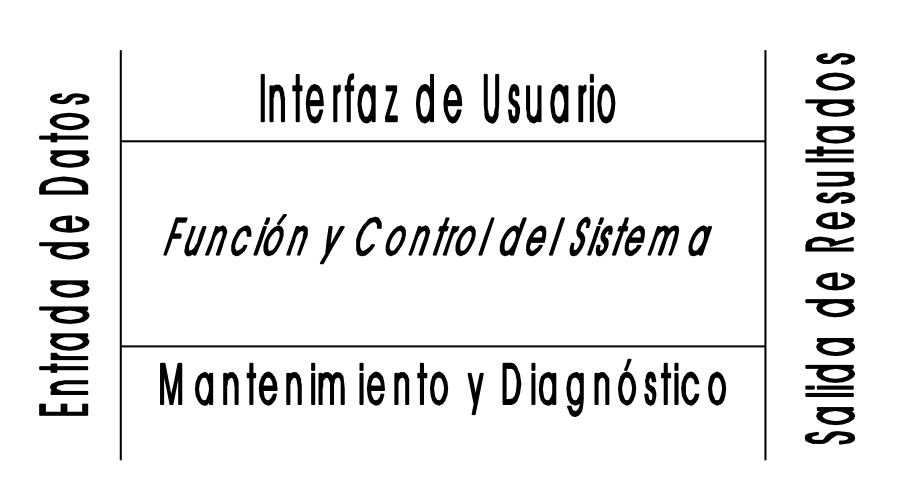
\includegraphics[width=0.6\linewidth]{Resources/Tema4/diagramaArquitectura.png}
    \caption{Diagrama de arquitectura de un sistema.}
\end{figure}

Si la complejidad del sistema lo requiere, puede formarse una jerarquía de niveles en la que el nivel superior se represente el sistema mediante un \uline{diagrama de contexto} (es el diagrama de arquitectura), y se irá detallando en sucesivos \uline{diagramas de flujo} (especifican el flujo de información en los subsistemas).

\begin{itemize}
    \item \textbf{Diagrama de contexto}: Representa el sistema en relación con su entorno, definiendo sus límites, y mostrando todos los productores y consumidores de información. Para ello, el sistema se encuentra en el centro del diagrama mientras que, a su alrededor, se sitúan las entidades o agentes externos, en sus correspondientes regiones, con los que el sistema se relaciona mediante flujos de información.
        \begin{figure}[H]
            \centering
            \includegraphics[width=0.5\linewidth]{Resources/contextdiagram}
            \caption{Ejemplo de diagrama de contexto.}
            \label{fig:diagramaDeContexto}
        \end{figure}
    \item \textbf{Diagrama de flujo de arquitectura}: Determinan el flujo de entre los diferentes \uline{subsistemas} a través de diagramas de flujo convencionales. Cada subsistema puede dar lugar a un diagrama de flujo, que pueden ser descompuestos a su vez en nuevos subsistemas, y ocupa una región del diagrama dependiendo de cuál sea su función (adquisición de datos, salida de datos, intefaz, etc.).
        \begin{figure}[H]
            \centering
            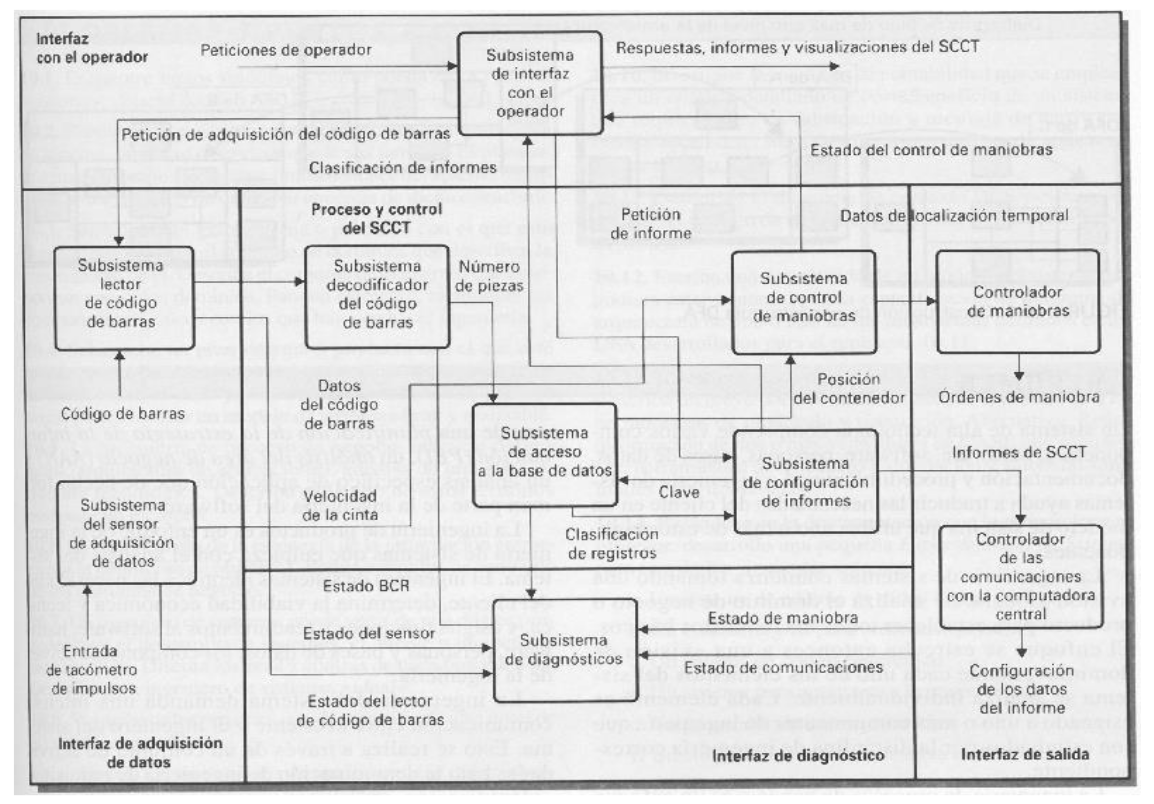
\includegraphics[width=0.8\linewidth]{Resources/Tema4/diagramaFlujo.png}
            \caption{Ejemplo de diagrama de contexto.}
            \label{fig:diagramaDeContexto}
        \end{figure}
\end{itemize}

\textbf{Nota:} \textit{Debe mantenerse la \uline{consistencia} entre los diagramas de distinto nivel. Al expandir un determinado subsistema en un diagrama de flujo, los flujos de información que conectan dicho subsitema con otros o con agentes externos deben figurar también. Estos flujos tendrán un extremo libre, que será el que los conectaba con dichos elementos que quedan fuera del ámbito del nuevo diagrama de flujo.}\\

\textbf{Nota:} \textit{Un diagrama de flujo de arquitectura no es un DFD, a pesar de las similitudes que puedan presentar, ya que este último se encuentra destinado a uso exclusivo para software.}

\section{Especificación del sistema}

Es un documento que sirve de base para analizar más adelante cada uno de los componentes que intervienen en el sistema, sean hardware, software o personas. Para ello, se describe \textbf{la función, rendimiento y restricciones que debe cumplir el sistema, limitando e indicando también el papel e interfaz de cada uno de sus componentes}.\\

Este documento debería permitir al cliente comprobar si el análisis del ingeniero del sistema satisface sus necesidades, por lo que debe ser revisado de forma conjunta para comprobar si:

\begin{itemize}
    \item Se ha delimitado correctamente el ámbito del proyecto.
    \item Se han definido correctamente la funcionalidad, las interfaces y el rendimiento.
    \item Las necesidades del usuario y el análisis de riesgos justifican el desarrollo.
    \item El cliente y el analista tienen la misma percepción de los objetivos del proyecto.
\end{itemize}

Además de la evaluación con el usuario, debe realizarse una evaluación técnica para determinar si:

\begin{itemize}
    \item Las estimaciones de riesgos, coste y de agenda son correctas.
    \item Todos los detalles técnicos (funciones, interfaces\ldots) están bien definidos.
    \item La especificación sirve como base para las fases siguientes.
\end{itemize}

% La siguiente sección no aparece en las presentaciones ¿?
\section{Análisis de requisitos del software}

Como resultado de la fase de análisis de requisitos del sistema, el componente de software tiene ahora asignados una función y rendimiento. Es ahora tarea del ingeniero de software el desarrollar, o adquirir si existen alternativas en el mercado, los componentes software para ello.

\subsection{Objetivos y actividades}

El análisis de requisitos del software tiene como objetivo \textbf{desarrollar una representación del software que pueda ser revisada y aprobada por el cliente}, y que sirva de enlace entre la asignación de funciones al software realizada, y el posterior diseño del software.\\

Desde el punto de vista del analista de sistemas, esta fase \textbf{define con mayor precisión} las funciones y rendimiento del software, las interfaces con otros componentes y las restricciones que debe cumplir. Desde el punto de vista del diseñador, este análisis \textbf{proporciona una representación} de la información, la función y el comportamiento del sistema que él se encargará de \textbf{traducir en un diseño de datos y programas}. Además, el análisis de requisitos permite a todos, incluido el cliente, valorar la calidad del software una vez haya sido construido, o incluso antes de ello.\\

\textbf{Nota:} \textit{El analista debe centrarse en el \textbf{qué}, no en el \textbf{cómo}}.\\

\textit{Pressman} propone que el análisis de requisitos del software puede dividirse en cinco áreas:

\begin{itemize}
    \item \textbf{Inicialmente, el analista estudia la especificación del sistema para comprender el papel del software dentro de este}, para ir definiendo y refinando los flujos y la estructura de la información, la función del programa y su papel, así como las interfaces y restricciones.
    \item Con este conocimiento, \textbf{se proponen y evalúan diferentes soluciones al problema}, hasta que se acuerda una solución con el cliente, y se puede especificar así el software de forma adecuada para que se puedan efectuar las siguientes fases de desarrollo.
    \item La \textbf{síntesis de modelos} que se realiza, además de permitir entender mejor los flujos de información y la función de cada elemento del software, dará pie a modelos que sirvan de \textbf{base para el diseño de software}, así como que puedan ser empleados para la creación de prototipos.
    \item La \textbf{especificación del software debe indicar qué es lo que debe hacer}, pero no cómo debe hacerlo. Pueden figurar características como el rendimiento, protocolos, estándares, soporte de hardware\ldots
    \item Será necesario \textbf{revisar la especificación}, dado que inicialmente será un documento ambiguo, incompleto, incorrecto e inconsistente.
\end{itemize}

\subsubsection{Principios del análisis de requisitos del software}

Por una parte, los dos primeros puntos se refieren a representar el sistema y la información que maneja mediante diagramas o representaciones textuales; por otra parte, los dos últimos se refieren a un método de trabajo \textit{top-down}.

\begin{enumerate}
    \item \textbf{Identificar y representar el ámbito de información del sistema}: La tarea que realiza el software consiste siempre en procesar información, pero esta puede estar representada tanto por \textbf{datos} (información que procesa el sistema) como por \textbf{sucesos o eventos} (cuándo debe procesarse esa información). Así, el ámbito de información admite dos puntos de vista: flujo de datos y flujo de control; de todos modos, en ambos casos se requiere concretar el contenido de la información, su estructura y el flujo.
    \item \textbf{Modelar la información, la función y el comportamiento del sistema}: Se emplean \textbf{modelos de datos} (información que transforma el software), \textbf{modelos de procesos} (funciones que transforman la información) y \textbf{modelos de control} (comportamiento del sistema). Los modelos se utilizan para comprender mejor lo que se quiere construir, dado que:
          \begin{itemize}
              \item Ayudan al analista a entender la información, función y comportamiento del sistema.
              \item Sirven de base para el trabajo del diseñador.
              \item Sirven para validar el producto una vez desarrollado.
          \end{itemize}
    \item \textbf{Descomponer el problema de forma que se reduzca la complejidad}: Para abordar problemas que son demasiado grandes o complejos.
    \item \textbf{Avanzar desde lo más general a lo más detallado}: Descomponiendo un problema en subproblemas, y definiendo modelos sobre cada uno, conformando una jerarquía de modelos.
\end{enumerate}
% Fin de la sección


\section{Especificación del software}

La especificación del software es el documento que culmina el análisis de requisitos, conteniendo una \textbf{descripción detallada} del ámbito de información, funciones y comportamiento asignados al \textbf{software}, así como \textbf{información sobre requisitos} de rendimiento, restricciones diseño, y sobre las pruebas a realizar una vez se haya construido el software (de aceptación).

\subsection{Principios de especificación}

\textit{Pressman} propone los siguientes principios a seguir en la especificación del software:

\begin{enumerate}
    \item \textbf{Debe modelar el dominio del problema}: Debe describir el sistema tal y como es percibido por los expertos del dominio de aplicación.
    \item \textbf{Es necesario separar funcionalidad e implementación}: El \textit{qué}, y no el \textit{cómo}.
    \item \textbf{El lenguaje de especificación debe estar orientado al proceso}: El sistema debe considerar la posibilidad de modificar su comportamiento por interacturar en un entorno dinámico.
    \item \textbf{Debe abarcar todo el sistema del que el software es parte}: El comportamiento de una parte, como lo es el software, solo puede ser definido en el contexto del sistema completo.
    \item \textbf{Debe abarcar también el entorno del sistema}: Siguiendo el principio anterior. Permite además describir la interfaz del sistema, del mismo modo que sucede con las interfaces de los componentes del mismo.
    \item \textbf{La especificación debe ser operativa}: Debe servir para determinar si una implementación concreta la satisface.
    \item \textbf{Debe ser ampliable y tolerante a la incompletitud}: Al ser una especificación un modelo de un sistema real, nunca será completa (\textit{desde luego, será extremadamente difícil conseguirlo}), pero puede desarrollarse de forma incremental, a distintos niveles de detalle.
    \item \textbf{Debe estar localizada y débilmente acoplada}: La especificación sufrirá continuas modificaciones, por lo que su estructura debe facilitarlas todo lo posible. 
\end{enumerate}

\subsubsection{Características del documento de especificación}

En cambio, \textit{Piattini} propone una serie de características que debe cumplir la especificación para ser un documento útil:

\begin{enumerate}
    \item \textbf{No ambigua}: Cada característica del producto debe ser descrita con un término único y, en los casos en que un término se use en distintos contextos por distintos significados, debe incluirse un \textbf{glosario}. El uso del lenguaje natural implica un gran riesgo por su ambigüedad inherente.
    \item \textbf{Completa}: Una especificación de requisitos software (\textbf{ERS}) está completa si:
          \begin{itemize}
              \item Incluye todos los requisitos significativos del software.
              \item Define la respuesta software a todas las posibles entradas en todas las posibles situaciones.
              \item Está conforme con cualquier estándar de especificación que se deba cumplir.
              \item Están etiquetadas y referenciadas todas las tablas, figuras y diagramas del texto, y están definidos todos los términos y unidades de medida.
              \item No contiene la expresión \textit{TBD} (por determinar). Sin embargo, hay veces es necesario utilizarla, y debe acompañarse de:
                    \begin{itemize}
                        \item Una descripción de las condiciones que han causado el \textit{TBD}.
                        \item Una descripción de qué hay que hacer para eliminar el \textit{TBD}.
                    \end{itemize}
          \end{itemize}
    \item \textbf{Fácil de verificar}. Cualquier requisito al que hace referencia se puede verificar mediante algún procedimiento finito y efectivo en coste.
    \item \textbf{Consistente}: Si, y solo si, ningún conjunto de requisitos descritos en ella son contradictorios, total o parcialmente. Se pueden presentar tres tipos distintos de conflictos:
        \begin{itemize}
            \item Se define el mismo objeto real pero con distintos términos para designarlo.
            \item Las caracerísticas especificadas para objetos reales están en conflicto; \textit{por ejemplo: luces azules vs. luces verdes}.
            \item Hay un conflicto lógico o temporal entre dos acciones; \textit{por ejemplo: sumar dos valores vs. multiplicarlos.}
        \end{itemize}
    \item \textbf{Fácil de modificar}: Estar apropiadamente organizada, y no contener redundancia.
    
    \textbf{Nota:} \textit{La redundancia en sí no es un error, pero puede conducir fácilmente a ello. Es mejor emplear referencias cruzadas en su lugar.}
    \item \textbf{Facilidad para identificar el origen y las consecuencias de cada requisito}: De este modo, cuando se debe llevar a cabo una modificación, pueden determinarse claramente los requisitos que pueden verse afectados por ellas. Se consigue estableciendo la \uline{trazabilidad}.
    \item \textbf{Facilidad de utilización durante la fase de explotación y mantenimiento}:
        \begin{itemize}
            \item Si el personal que encarga del mantenimiento no ha estado relacionado con el desarrollo del producto, y debe llevar a cabo modificaciones ``profundas'', es necesario actualizar la documentación de diseño y de los requisitos. Por ello, además de que la ERS debería ser fácilmente modificable, debería contar con un registro de las características especiales de cada componente, como criticidad u origen, para facilitar dichos cambios; \textit{es decir, será mejor poder disponer de toda la información posible para evitar cometer errores.}
            \item Podría darse el caso de que parte de la información necesaria para el mantenimiento se dé por supuesta en la organización del desarrollo y, si la organización del mantenimiento no cuenta con ella, supondrá un gran problema.
        \end{itemize}
\end{enumerate}

\textbf{Nota:} \textit{Al igual que sucede con la especificación del sistema, la especificación de requisitos del software debe ser revisada conjuntamente por el cliente y el ingeniero del software. En primera instancia, debe determinarse si el sistema cumple, según el papel aquí especificado para el software, con la función, restricciones y rendimiento requeridos por el cliente, y ver si es necesario cambiar algunas de las estimaciones de coste, riesgo o agenda. En segundo lugar, debe realizarse una revisión mucho más detallada para detectar imprecisiones o ambigüedades en la especificación.}


\section{Verificación y Validación de requisitos}

La \textbf{validación de los requisitos es la que permite mostrar} (verificar) que éstos son los que \textbf{definen el sistema que el cliente desea}.\\

Presenta una relativa similitud con el análisis, ya que implica encontrar problemas con los requisitos, pero disciernen en que la validación comprende un bosquejo completo del documento de requisitos, mientras que el análisis implica trabajar con requisitos incompletos.

\subsection{Estrategias}

Durante el proceso de validación, deben llevarse a cabo diferentes tipos de comprobaciones sobre los requisitos:

\begin{enumerate}
    \item \textbf{Comprobación de validez}. Dado que cada sistema tendrá sus propias necesidades, ¿la especificación responde a todas las necesidades del proyecto? \textit{Por ejemplo: es posible que se identifique una necesidad de contar con determinadas funciones adicionales a medida que los analistas comprenden mejor el sistema que el cliente desea.}
    \item \textbf{Comprobación de consistencia}: Los requisitos en el documento no deben contradecirse.
    \item \textbf{Comprobación de totalidad}: Se deben incluir requisitos que definan todas las funciones y restricciones propuestas para el sistema.
    \item \textbf{Comprobación de realismo}: Asegurar que los requisitos puedan implementarse actualmente, y teniendo en cuenta además restricciones de presupuesto y calendarización.
    \item \textbf{Verificabilidad}: Debe ser posible diseñar un conjunto de verificaciones (pruebas) para demostrar que el sistema a entregar cumple los requisitos.
\end{enumerate}

\subsection{Técnicas}

Las técnicas dictan cómo llevar a cabo las estrategias:

\begin{enumerate}
    \item \textbf{Revisiones de requisitos}: Varios implicados, pertenecientes tanto al cliente como al contratista, llevan a cabo un proceso de análisis sistemático del documento de requisitos para encontrar anomalías y omisiones.
    \item \textbf{Construcción de prototipos}: Se muestra un modelo ejecutable del sistema a los usuarios finales para que experimenten y comprueben si cumple sus necesidades.
    \item \textbf{Generación de casos de prueba}. Los requisitos deben poder probarse. Si una prueba es difícil o imposible de diseñar, suele significar que los requisitos serán difíciles de implementar, por lo que deben ser reconsiderados.
    \item \textbf{Análisis de consistencia automática}. Si los requisitos se expresan en una notación estructurada o formal.
\end{enumerate}

\textbf{Nota:} \textit{No deben menospreciarse las dificultades en la validación de requisitos, dado que es difícil demostrar que un conjunto de requisitos cumple las necesidades del usuario, por requerir visualizar cómo el sistema final encajaría en su entorno de explotación; esto será complejo para los profesionales de la computación, pero aún más para los usuarios. Por ende, la validación de requisitos probablemente descubrirá todos los problemas en las interpretaciones realizadas sobre las necesidades del cliente, y será inevitable corregir todos estos problemas.}


\section{Administración de requisitos}

La \textbf{ERS habitúa ser un proceso iterativo}, como consecuencia del progreso del producto de software; a fin de cuentas, es \textbf{casi imposible especificar algunos detalles en el momento que se inicia el proyecto}. También es muy probable que se realicen cambios adicionales como resultado de haber encontrado deficiencias.\\

Dos consideraciones a tener en cuenta en este proceso son:

\begin{itemize}
    \item Especificar los requisitos de la forma más completa posible, a pesar de que se prevean de forma inevitable revisiones en él.
    \item Debe iniciarse un proceso de gestión formal del cambio, para identificar, controlar, seguir e informar de posibles cambios tan pronto como sean identificados. De este modo, se podrá contar con un rastreo preciso de las modificaciones de la ERS, así como discernir entre los fragmentos actuales de la ERS y sus anteriores versiones.
\end{itemize}

Como se puede ver, la administración de requisitos es el proceso de comprender y controlar los cambios en los requisitos del sistema. Consta de \textbf{dos etapas}: la planificación debería comenzar al mismo tiempo que la obtención de requisitos inicial, y la administración activa debe comenzar tan pronto como esté lista la primera versión del documento de requisitos.

\subsection{Clasificación cualitativa}

Desde una perspectiva evolutiva, los requisitos son de una de las siguientes dos clases:

\begin{itemize}
    \item \textbf{Requisitos duraderos}: Relativamente estables dado que derivan de la actividad de la organización y, por lo tanto, están relacionados directamente con el dominio del sistema. \textit{Por ejemplo: en un hospital siempre habrá pacientes, doctores\ldots}
    \item \textbf{Requisitos volátiles}: Probablemente cambiarán durante el desarrollo del sistema o después de que se haya puesto en operación. \textit{Por ejemplo: por cambios en las políticas gubernamentales de salud}.
    
    \textit{Sommerville} clasifica estos últimos en:
    \begin{itemize}
        \item \textbf{Cambiantes}: Debido al ambiente en que opera la organización.
        \item \textbf{Emergentes}: Surgen al incrementarse la compresión del cliente en el desarrollo del sistema; dicho de otro modo, \textit{se entiende más sobre lo que el cliente desea}.
        \item \textbf{Consecutivos}: Son resultado de la introducción del sistema en su entorno de explotación (puede suponer cambios en los procesos de la organización).
        \item \textbf{De compatibilidad}: Dependen de sistemas particulares o procesos de negocios dentro de la organización.
    \end{itemize}
\end{itemize}

\subsection{Clasificación cuantitativa}

Desde otro punto de vista, simplemente pueden clasificarse asignándoles el \textbf{valor de estabilidad} que se considere apropiado: baja, media y alta.

\subsection{Planificación de la administración de requisitos}

La administración de requisitos es muy cara, por lo que es necesario definir en todo proyecto el nivel de detalle necesario para este proceso. Para ello, deben concretarse los siguientes aspectos:

\begin{itemize}
    \item \textbf{La identificación de requisitos}: Cada requisitos debe ser identificable de forma unívoca.
    \item \textbf{Un proceso de administración del cambio}: Conjunto de actividades que evalúan el impacto y costo de los cambios.
    \item \textbf{Políticas de rastreo}: Definen las relaciones entre requisitos dependientes, entre requisitos y los módulos del diseño en los cuales serán implementados, y entre los requisitos y sus fuentes (quién y por qué se propusieron). Esto permite que, cuando un cambio sea propuesto, se pueda rastrear el impacto en los requisitos y en el diseño, de modo que se pueda valorar si proceder a realizar el cambio o no.
    \item \textbf{Ayuda de herramientras CASE} (\textit{Computer Aided Software Engineering}).
\end{itemize}

\textbf{Nota:} \textit{Es habitual registrar esta información de rastreo mediante matrices de rastreo. Además, la administración de requisitos idealmente recurrirá a la ayuda de herramientas CASE para almacenarlos, y administrar sus cambios y trazabilidad.}

\subsection{Administración del cambio de requisitos}

Esta administración se aplica a todos los cambios propuestos en los requisitos. La ventaja de emplear un proceso formal es que todos los cambios propuestos son tratados \textbf{de forma consistente} y que los cambios en el documento de requisitos se realizan \textbf{de forma controlada}.\\

\textbf{Nota:} \textit{La gestión del cambio es un proceso aparte para todos los artefactos del proyecto, pero los primeros sobre los que se aplica son los requisitos.}\\

Existen tres etapas principales:

\begin{itemize}
    \item \textbf{Análisis del problema y especificación del cambio}: Tras \textbf{identificar un problema}, o a veces recibir una \textbf{propuesta de cambio}, se analiza la información correspondiente para verificar que es válida y, entonces, se hace una propuesta de cambio de requisitos más específica.
    \item \textbf{Análisis del cambio y costeo}: Se valora el efecto de un cambio propuesto empleado la información de rastreo y el conocimiento general de los requisitos del sistema. Finaliza con la toma de decisión de si procede o no el cambio.
    \item \textbf{Implementación del cambio}: Se modifica el documento de requisitos y, si procede, el diseño e implementación del sistema.
\end{itemize}

En caso de que se requiera de forma urgente un cambio en los requisitos del sistema, existirá la tentación de hacer el cambio del sistema y de modificar el documento tras ello. Esto conduce, inevitablemente, a que la especificación de requisitos y el sistema se desfasen, de modo que no sean consistentes el uno con el otro por, por ejemplo, posponer la actualización del documento.
